\chapter{Experiments and Evaluations\label{cha:chapter4}}

To evaluate the Frankenbot's modular architecture on the basis of the user experience, the surveys has been conducted. 
\\~\\
For accomplishment of this research, random users were selected irrespective of their profession, studies background and any race or gender discrimination. But the age limit constraint was set to be above 18. As participants were considered to be accused of a robbery and have to chat with a detective bot and answer his questions which can be a bit rude and straight forward for youngsters below 18. So the participant with the minimum age was 22. On contrary, the one with the maximum age was 34. And the average age calculated as 25.65 with the standard deviation of 2.37. Visuals have been shown in the Figure \ref{fig:ageGraph}.

\begin{figure}[!h]
    \centering
    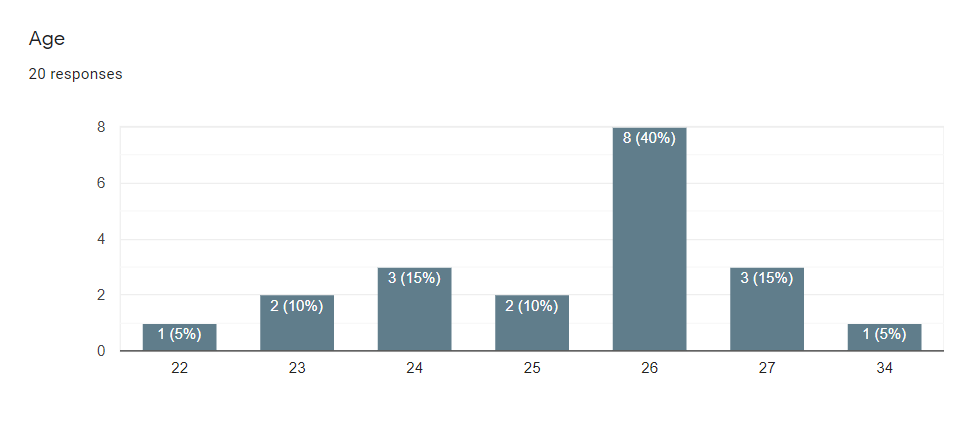
\includegraphics[width=0.9\textwidth]{img/Age_Graph.PNG}
    \caption{Age stats of participants}
    \label{fig:ageGraph}
\end{figure}
\\~\\
Total 20 users participated in this study. Most of them appeared to be from technical background as maximum of them were students from different universities. Secondly, majority of participants revealed themselves to be IT employees other than the students. While remaining revealed themselves as engineer, teacher and business qualified. More details have been shown in the Figure \ref{fig:profGraph}.

\begin{figure}[!h]
    \centering
    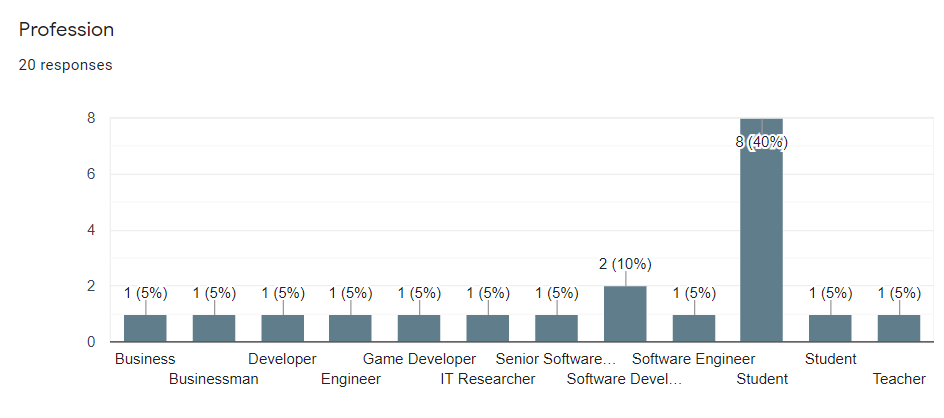
\includegraphics[width=0.9\textwidth]{img/Profession_Graph.PNG}
    \caption{Profession related details of participants}
    \label{fig:profGraph}
\end{figure}

\section{Conducted Surveys}
All participants were asked to complete two surveys. One named as "Frankenbot's Experience Survey" was designed with the help of \cite{MOLLER200726}\cite{itut}. For the second survey, the standardized tool to personally evaluate the usability and design of an interactive product known as AttrakDiff\cite{attrakdiff} has been used. First survey was designed using Google Forms and the purpose of it was to capture the user's interaction experience about the Frankenbot. While, the purpose of AttrakDiff's study was to evaluate different aspects such as Frankenbot's utility and usability. Furthermore, it also helped to weigh the chatbot for task-oriented and self-oriented qualities. 
\\~\\
The users were provided with the link to the deployed chatbot's interface as a web page and they can easily access it from their own places. It provided ease to the user and enhanced the comfortability factor for them. Also, they have to read the description and instructions provided for them on the web page. And they have to figure out what to do and how to operate the chatbot on their own without any external help. Which has given more realistic and unbiased essence to the results obtained.
\\~\\
For the surveys, the web page contains the heading as "Frankenbot's Request" in which the users were requested to complete the surveys once, they are finished having chat for a fun purpose with the chatbot. They have been provided with the links to both surveys.
\\~\\
The surveys were conducted in English language. Whereas, AttrakDiff's survey has the option for both English and German. You can find the "Frankenbot's Experience Survey" in the Appendices \ref{appen:survey}. Furthermore, AttrakDiff's Single Evaluation Study\cite{indeval} has been used as the second survey.
\\~\\
The questionnaires were filled by the participants on their own devices. As link to the deployed chatbot has been shared with them using different social platforms along with an introductory text about the purpose of the study. When the user was interacting with the chatbot all communication was getting stored in the log file for the future records and usage.

\section{Experimental Setup}
This research study has been conducted to gather the results for what user has experienced while interacting with the chatbot. The whole experiment itself has been divided in to four major parts mentioned below:
\begin{enumerate}
    \item Explanation of the chatbot for the participants in order to make its testing successful.
    \item Participants were requested for accomplishing set of tasks with the chatbot.
    \item The questionnaire to collect the user's interaction experience about the chatbot named as "Frankenbot's Experience Survey".
    \item Quality evaluation of the chatbot via AttrakDiff's Single Evaluation.
\end{enumerate} 
All of these are explained underneath in detail.

\subsection{Explanation of the Chatbot}
Users were provided with the description and instructions on the web page about the chatbot. The following sub-sections contain the required information and directions to for the users to operate the chatbot. Visual representation has been displayed in the Figure \ref{fig:userInter}.

\subsubsection*{Information}
The participants were provided with the introduction about the Frankenbot that it is the detective chatbot designed to interrogate you about the armed robbery happened few days back at a spatkauf near Berliner Strasse. It is responsible for investigating, so it is going to ask you some questions to come up with a decision. It will include, what it has investigated so far. Also you can have general conversation with it like you can ask it to talk about general stuff with you, about corona virus and its stats, to make you laugh, to do gossips, how does it feel, who is it, what does it eat and other related questions about the chatbot. You can switch between the topics at any moment as it is designed for parallel handling of the multiple topics. Kindly, communicate with it until it reaches any decision or says you goodbye before you jump to completion of the surveys.
\\~\\
Lastly, the ending of the information provided a brief note about how to re-initiate the chat. If user gets lost in between the dialogue and want to reinstate the detective game then just send a greeting message (hi, hello etc.) and the chatbot will restart it for him/her.

\subsubsection*{Instructions}
The user was asked to think as he/she is accused of a robbery and sitting in front of a detective and have to answer his brutal and tricky questions in order to prove his/her innocence. Otherwise, he/she will be declared as a culprit. It is a responsibility of a detective to make a decision based on user's answers to his questions.
\\~\\
At the end of the instructions there was a small notice available for the user to remove his/her doubts about its reality that it is the fictional detective chat bot designed only for testing and fun purpose.

\subsection{Tasks}
The participants were requested to accomplish following tasks beforehand, to fill the surveys.
\begin{itemize}
    \item Users were requested to play a small game with the detective chatbot and answer the questions, the way they wanted.
    \item They were also requested to have general dialogue with the chatbot. Ask it to talk about general stuff, about corona virus and its stats, to tell a joke, to do gossips, queries about its feelings and emotions and other related questions.
    \item Additionally, they were also asked to switch the topics. Means, they should start talking about general stuff if they are talking to the detective bot and vice versa by just replying to the last question of the previous topic.
    \item Lastly, they were requested not to leave the conversation in between until they reach the ending of the detective game. 
\end{itemize} 
\\~\\
All users were requested to chat with the chatbot at minimum, until it came up with any decision or says them goodbye. Other than that, there was no time restriction for them and they could have a dialogue for as long as they desired to.

\subsubsection*{Frankenbot's Request}
Finally, the user was requested that once he/she has finished having fun with the chatbot, please don't forget to complete two of the assessments provided as the links. The links were disabled when the web page gets loaded and gets activated after 1 minute, so that in meanwhile the user should get familiar with the chatbot by doing some chat with it. Frankenbot also stated that it welcomes and highly appreciates your prestigious feedback which will help its developer to get it evaluated and enhance its abilities for your better experience.

\subsection{Frankenbot's Experience Survey}
When the user successfully completed the tasks allocated to him/her. Then he/she filled out the survey about his/her interaction with the chatbot. The questionnaire itself has been divided in to the following sections:
\begin{itemize}
    \item Users overall impression about the interaction with the chatbot.
    \item Familiarity of the user with the already existing chatbots.
    \item Whether the user succeeded to achieve the desired goals.
    \item How was the communication with the chatbot.
    \item What was the behaviour of the chatbot with the users.
    \item How well the dialogue was designed.
    \item Personal impression and user's experience about the chatbot.
    \item Users opinion about the chatbot's usability. 
\end{itemize} 
All sections have been consisted of several questions. And user has to respond by selecting an option out of linear scale from 1 to 5 whether he/she strongly agrees, agrees, undecided, disagrees or strongly disagrees with it. Most of the questions needed to be answered using these five options. Other than that overall impression about the chatbot has been measured using the linear scale of 5 options starting from 1 and ending on 5 as excellent, good, fair, poor and bad.

\subsubsection*{Overall Impression}
This section included a question about the user's overall impression about the interaction with the chatbot. It has been measured using the linear scale of 5 options starting from 1 and ending on 5 as excellent, good, fair, poor and bad. And out of the total 20 responses collected by the conduction of the survey, 2(10\%) responded with excellent mark and 9(45\%) rated it as good. So, total 11 out of 20 which is 55\% of the total participants, have passed positive remarks about it. Whereas, other 4(20\%) judged it as fair which also lies under the category of acceptable. So after summing up the percentages, 75\% of the participants rated their interaction as charming. On contrary, out of the remaining participants 3(15\%) rated it as poor and only 2(10\%) assigned it a bad label. So, it depicts that overall users impression about the interaction with the chatbot went well. For graphical representation of it, refer to the Figure \ref{fig:overallImpre}.

\begin{figure}[!h]
    \centering
    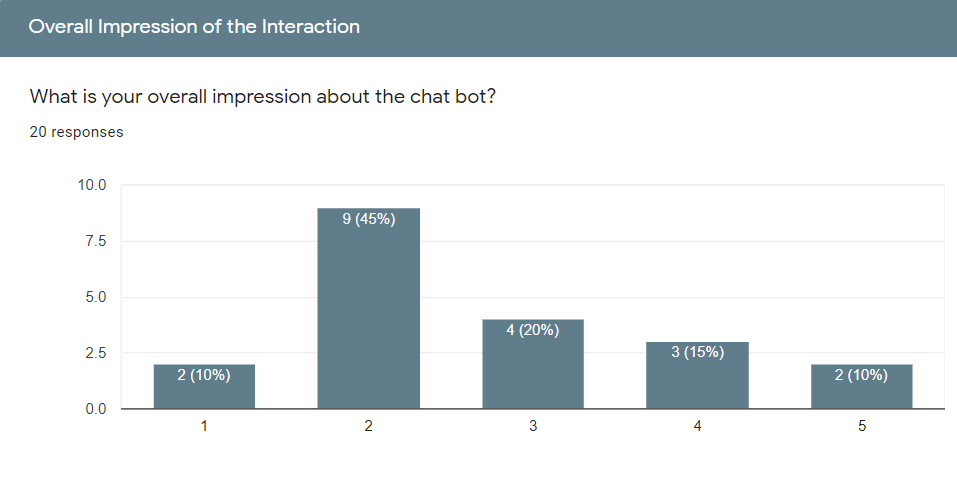
\includegraphics[width=0.9\textwidth]{img/Overall_Impression.PNG}
    \caption{Overall impression of the interaction with the chatbot}
    \label{fig:overallImpre}
\end{figure}

\subsubsection*{Familiarity with Existing Chat Bots}
This section added to the questionnaire just to figure out the experience of the participants with already existing chatbots that whether they are well familiar with the chatbots or are inexperienced with this emerging technology. So that, if majority of them have the good knowledge of any of the existing chatbots, it will provide more strength and solidity to the results gathered from such participants.
\\~\\
There were total 3 questions available under this section that participants have to answer:
\begin{enumerate}
    \item I feel that I am well familiar with the chat bots like Google Assistant, Apple's Siri etc. (Possible options lie between scale of strongly agree to strongly disagree).
    \item I communicate with the chat bots. And the possible options provided were Frequently (daily or several times in a week), Seldomly (rarely in weeks or months), Just few times and Never.
    \item Purpose of my chat bots usage is: (only if you answered question no. 2 positively). Possible answers could be any out of the followings: Personal commands to provide you assistance in performing tasks, For fun, Not feel lonely and No reason.
\end{enumerate}
Fortunately, for the first statement, 16(80\%) appeared to be well familiar with the existing chatbots. 2(10\%) answered with undecided and remaining 2(10\%) just disagreed with the statement but no one strongly disagreed with it. Graph depicting such results has been shown in the Figure \ref{fig:familiarity}. Coming to the second statement, 5(25\%) detected to be frequent users. 8(40\%) resulted to be the seldom users. Whereas, 6(30\%) communicated just few times with the chatbots as shown in the Figure \ref{fig:commChatRes}. Lastly, almost 60\% knew how to operate and give commands to the chatbot. And around 30\% appeared to use it for joy and fun purpose. These all stats and readings portrays that experienced users participated in this study. And results obtained from the study is trustworthy and reliable. 

\begin{figure}[!h]
    \centering
    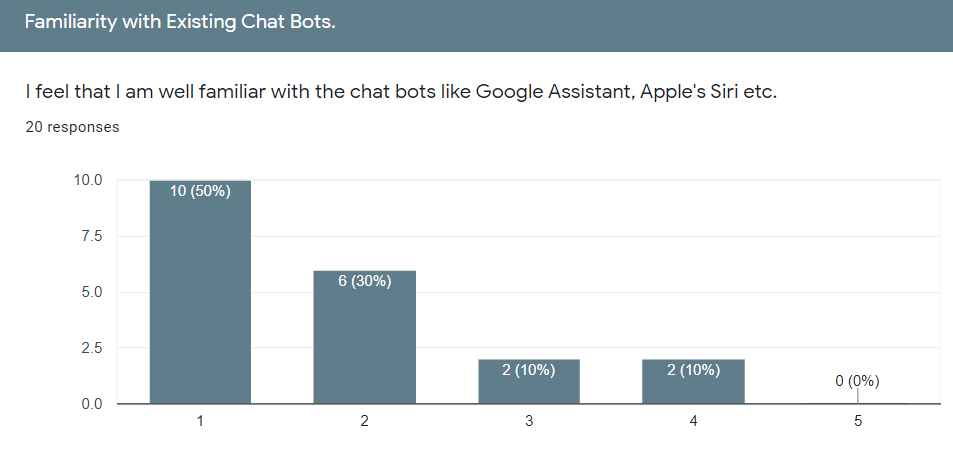
\includegraphics[width=0.9\textwidth]{img/Familiraity.PNG}
    \caption{Participants familiarity with the chat bots like Google Assistant, Apple's Siri etc.}
    \label{fig:familiarity}
\end{figure}

\begin{figure}[!h]
    \centering
    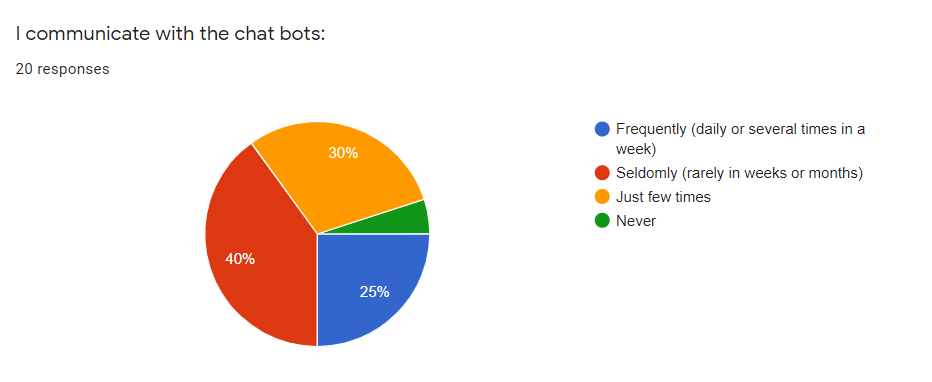
\includegraphics[width=0.9\textwidth]{img/Communicate_Chatbots_Result.PNG}
    \caption{Participants usage of the chat bots like Google Assistant, Apple's Siri etc.}
    \label{fig:commChatRes}
\end{figure}

\subsubsection*{Achievement of Goals}
It highlights whether the user succeeded to achieve the desired goals or not while having an interaction with the chatbot. It contained the following questions in respond to which user checked an option, including or in between of strongly agree to strongly disagree.
\begin{enumerate}
    \item The information provided by the chat bot was clear.
    \item The provided information was incomplete.
    \item The interaction with the chat bot was efficient.
    \item The chat bot is unreliable.
\end{enumerate}
Discussing the results and stats for the very first statement, 13(65\%) participants agreed upon the information provided by the chatbot was clear. Whereas, 3(15\%) were failed to decide about it. Only 4(20\%) just disagreed with it and no one strongly negated it. For better understanding of it just see the Figure \ref{fig:clearInfo}.

\begin{figure}[!h]
    \centering
    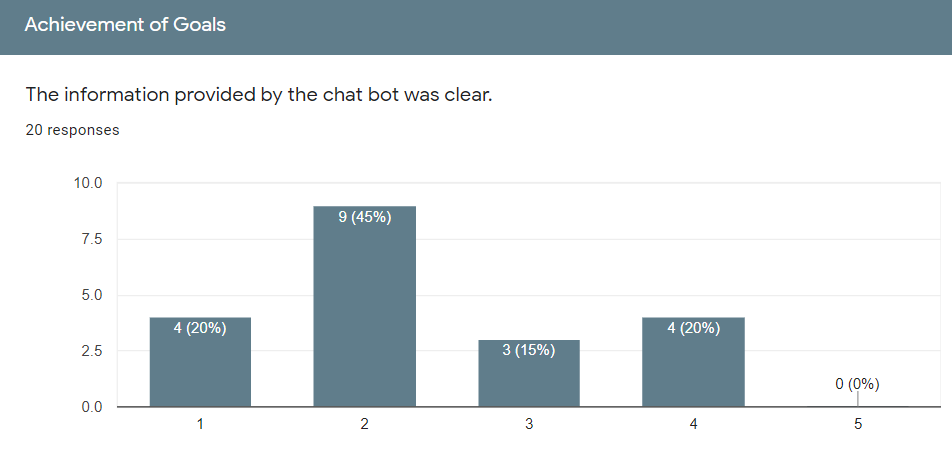
\includegraphics[width=0.9\textwidth]{img/Clear_Info.PNG}
    \caption{Stats depicting about the information provided by the chat bot was clear}
    \label{fig:clearInfo}
\end{figure}
\\~\\
For the second statement, 10(50\%) disagreed with it which tells that for them the provided information was complete. Whilst 7(35\%) were unable to make any decision about it. This is something can not ignored. It can happen due to various reasons: (i) due to lack of concentration (ii) misinterpretation of information or instructions (iii) chatbot responded falsely and the only reason for it could be a weakly trained Rasa's NLU due to limited training data. But still 50\% answered that the information was complete, so there are high chances that the reason lies somewhere between (i) and (ii). Visuals have been shown in the Figure \ref{fig:incompInfo}.

\begin{figure}[!h]
    \centering
    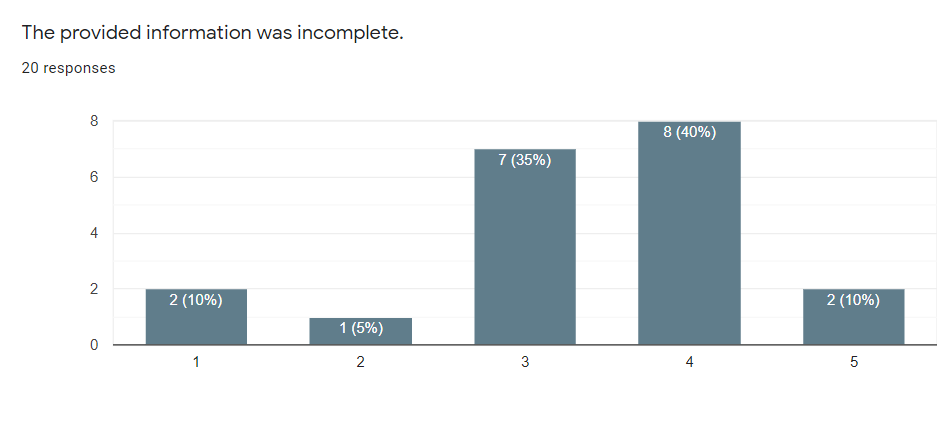
\includegraphics[width=0.9\textwidth]{img/Incomp_Info.PNG}
    \caption{Stats depicting about the provided information was incomplete}
    \label{fig:incompInfo}
\end{figure}
\\~\\
Moving to what has been concluded from the third statement seems to be something really positive. As 12(60\%) of the participants agreed upon the efficient interaction with the chatbot. Moreover, 4(20\%) failed to decide about it and only other remaining 4(20\%) disagreed with it. Refer to the Figure \ref{fig:effInt} for seeing the detailed graph of it.

\begin{figure}[!h]
    \centering
    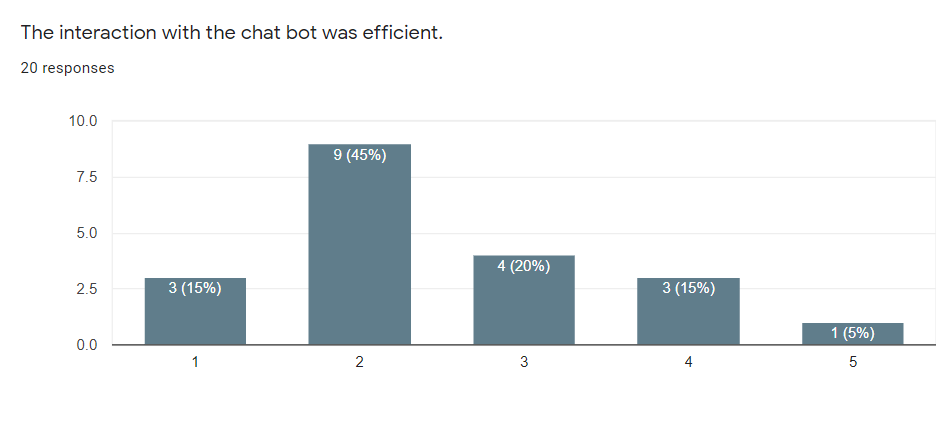
\includegraphics[width=0.9\textwidth]{img/Efficient_Inter.PNG}
    \caption{Stats depicting about the interaction with the chat bot was efficient}
    \label{fig:effInt}
\end{figure}
\\~\\
Lastly, forth statement stats are a bit disappointing. According to only 6(30\%) users, the chatbot was reliable. On contrary, 8(40\%) declared it unreliable and remaining 6(30\%) failed to take any decision about it. The possible reason for its unreliability could be its inability to respond the user for all of his/her queries. And it is happening due to limited data provided for training and also the demo chatbot was designed for limited use cases. In order to design a fully loaded chatbot that can reply to the user for any of his/her utterance, lot of training data and processing is required and within limited time and resources it was not possible. But, it could be done in future. See the Figure \ref{fig:unreliBot} for better understanding of results.

\begin{figure}[!h]
    \centering
    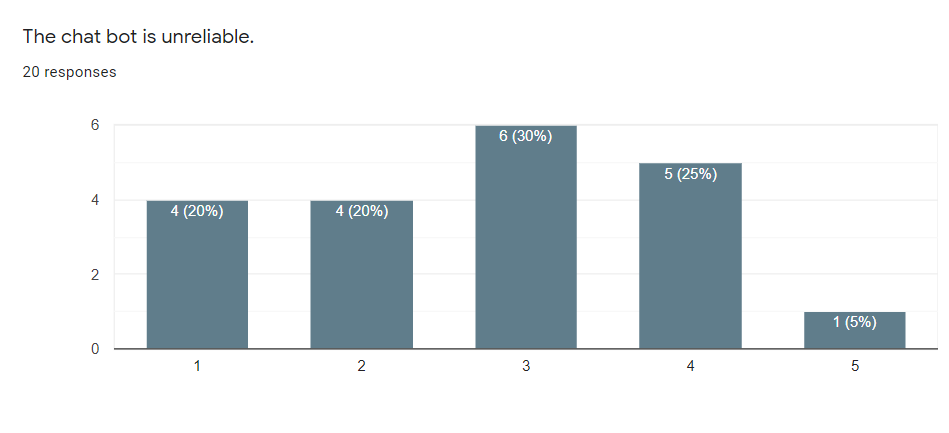
\includegraphics[width=0.9\textwidth]{img/Unreli_Bot.PNG}
    \caption{Stats depicting about the chat bot is unreliable}
    \label{fig:unreliBot}
\end{figure}

\subsubsection*{Communication with the Chat Bot}
The purpose of this section was to collect the user's opinion that how was the communication with the chatbot. It consisted of the following three questions:
\begin{enumerate}
    \item The chat bot understood my messages well.
    \item I always knew what to say to the chat bot.
    \item The interaction with the chat bot sounded natural.
\end{enumerate}
Total 10(50\%) of the participants disagreed with the statement that the chatbot understood their messages well. And 4(20\%) out of the remaining 10 were not able to decide about it. Remaining 6(30\%) answered positively with it. As majority disagreed with the statement and the possible reason could be that the chatbot responded incorrectly. And the only reason for it could be the problem with natural language understanding. It detected the wrong intent for the user utterance. Graphical representation can be found in the Figure \ref{fig:understWell}.

\begin{figure}[!h]
    \centering
    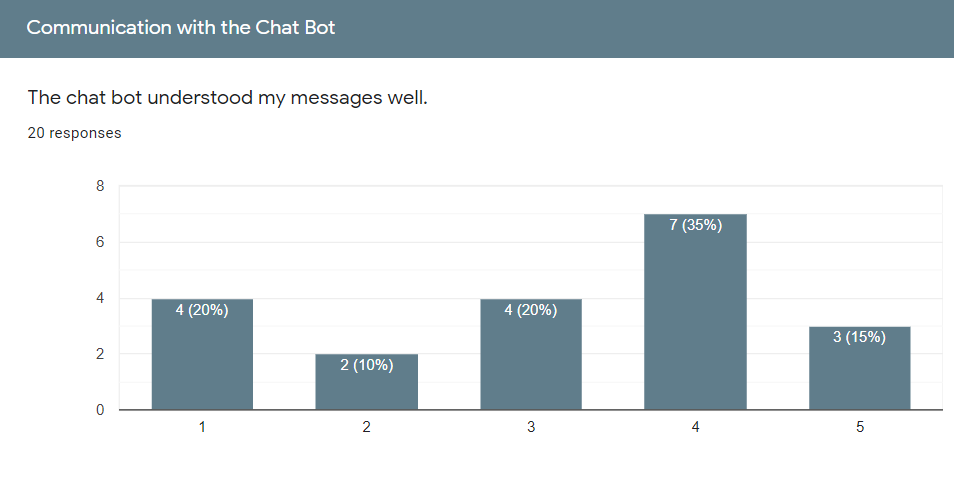
\includegraphics[width=0.9\textwidth]{img/Underst_Well.PNG}
    \caption{Responses for the statement that the chat bot understood messages well.}
    \label{fig:understWell}
\end{figure}
\\~\\
Coming towards the next statement, 12(60\%) agreed with it that they always knew what to reply or ask the chatbot. Other than those, 3(15\%) failed to make any decision about it and remaining 5(25\%) disagreed with it. Results have been displayed in the Figure \ref{fig:saytoBot}.

\begin{figure}[!h]
    \centering
    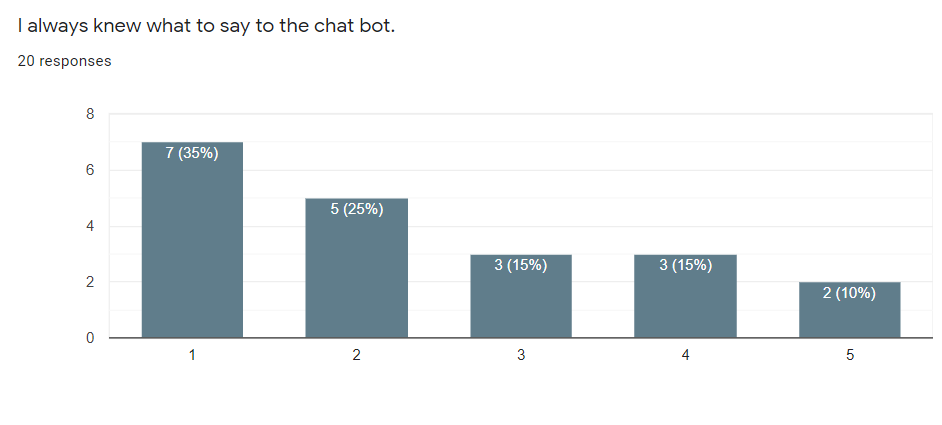
\includegraphics[width=0.9\textwidth]{img/Say_to_Bot.PNG}
    \caption{Responses for the statement that the user always knew what to say to the chat bot.}
    \label{fig:saytoBot}
\end{figure}
\\~\\
Responses for the third statement showed that 9(45\%) participants felt the communication as natural. Out of other 11 only 4(20\%) failed to decide about it. Along with that remaining 7(35\%) showed disagreement with it. And the reason could be the wrong intent detection by the NLU. For visuals look in to the Figure \ref{fig:naturalInter}.

\begin{figure}[!h]
    \centering
    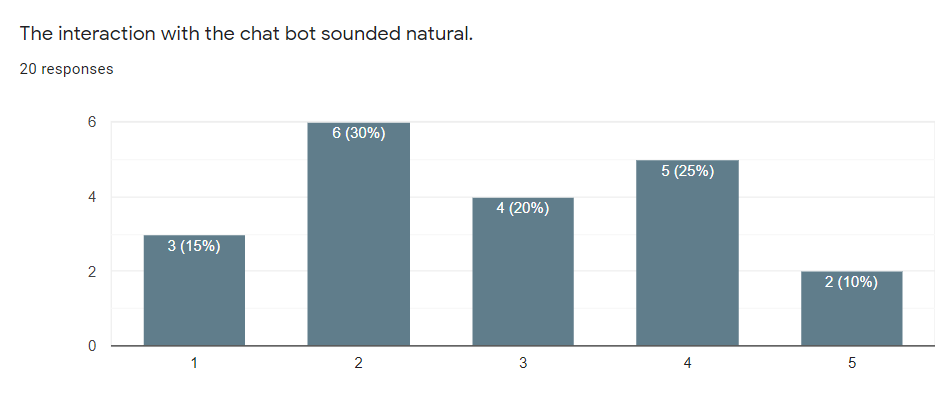
\includegraphics[width=0.9\textwidth]{img/Natural_Inter.PNG}
    \caption{Responses for the statement that the interaction with the chat bot sounded natural.}
    \label{fig:naturalInter}
\end{figure}

\subsubsection*{Behaviour of the Chat Bot}
Intentions behind adding this section to the questionnaire was to detect the behaviour of the chatbot with the user. It consisted of the seven questions answered by the user on the scale of agreement or disagreement as stated below: 
\begin{enumerate}
    \item The chat bot responded too slowly.
    \item The chat bot is friendly.
    \item The chat bot didn't always meet my expectations.
    \item I didn't always know what answer the chat bot is expecting from me.
    \item The chat bot made many errors.
    \item I was able to recover easily from errors. (only in case of errors).
    \item The chat bot behaved in cooperative way.
\end{enumerate}
Analysing the results for this section's initial statement, 16(80\%) strongly disagreed with it. Whereas, another 1(5\%) also negated the statement which makes the number total 17(85\%) who portrayed that the responding speed for the chatbot was fast enough as shown in the Figure \ref{fig:respSpeed}. 

\begin{figure}[!h]
    \centering
    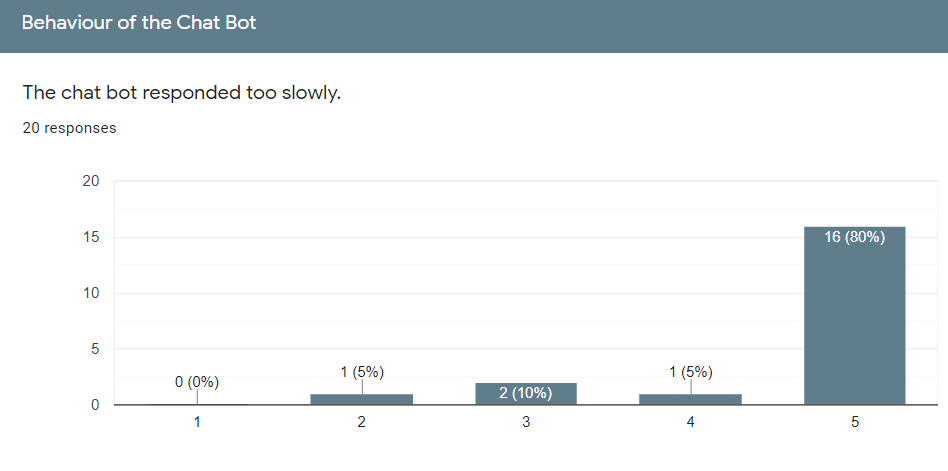
\includegraphics[width=0.9\textwidth]{img/Response_Speed.PNG}
    \caption{Result about the chat bot's response speed}
    \label{fig:respSpeed}
\end{figure}
\\~\\
Secondly, 10(50\%) rated the chatbot as friendly. While 7(35\%) other respondents were unable to come up with any decision about it as displayed in the Figure \ref{fig:friendlyBot}. It could be due to the reason that different persons have their own perception about friendliness. Also, the demo topic included the detective bot. So, it was meant to respond with straight forward statements. Which could be felt a bit offensive some times depending upon the user's nature. 

\begin{figure}[!h]
    \centering
    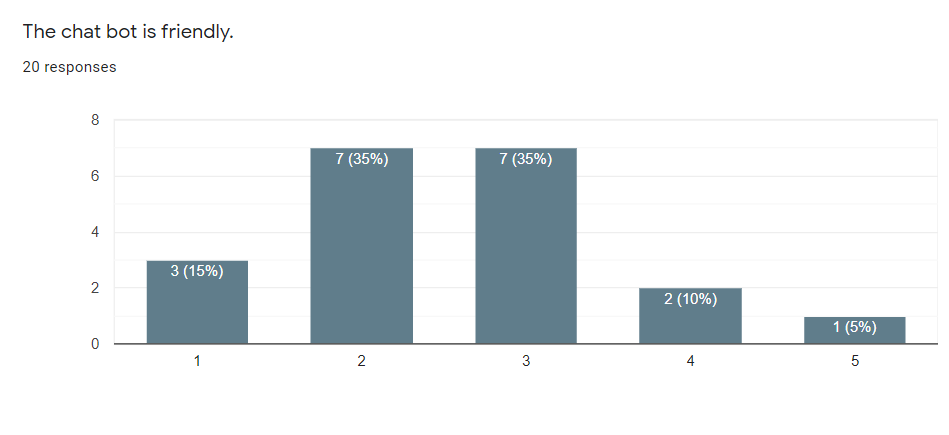
\includegraphics[width=0.9\textwidth]{img/Friendly_Chatbot.PNG}
    \caption{Result about the chat bot's friendliness}
    \label{fig:friendlyBot}
\end{figure}
\\~\\
Thirdly, the chatbot didn't meet the expectations for 9(45\%) of the participants. Additionally, other 6(30\%) were failed to determine about it and only 5(25\%) stated that it fulfilled their expectations and can be visualized in the Figure \ref{fig:botExpec}. So it can be clearly concluded from it that the chatbot failed to meet the users expectations. The possible reason for it might be same to the statement in the last section that the chatbot didn't understand the messages well.

\begin{figure}[!h]
    \centering
    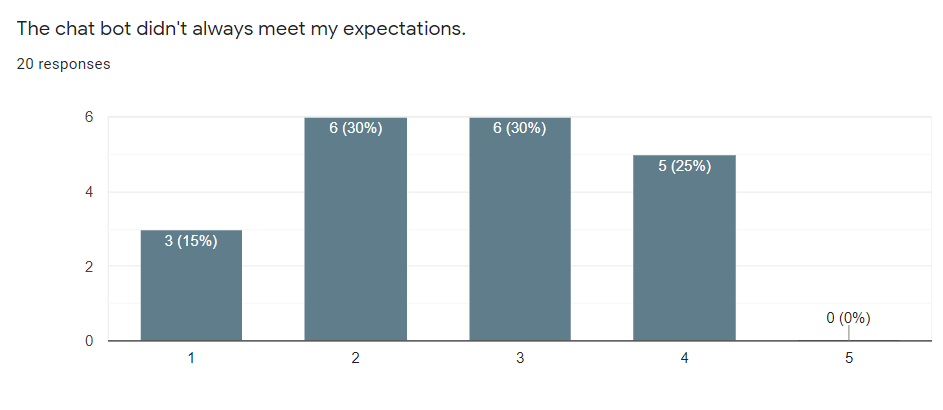
\includegraphics[width=0.9\textwidth]{img/Chatbot_Expect.PNG}
    \caption{Result for the expectations from the chat bot}
    \label{fig:botExpec}
\end{figure}
\\~\\
Reviewing the results for the forth statement, 11(55\%) of the respondents showed agreement with the statement that they didn't always know what answer was the chatbot expecting from them as displayed in the Figure \ref{fig:ansExpec}. It could be due to the limitation of the training data as the chatbot was just trained for limited intents but the users were provided with free choice to ask anything from the chatbot. 

\begin{figure}[!h]
    \centering
    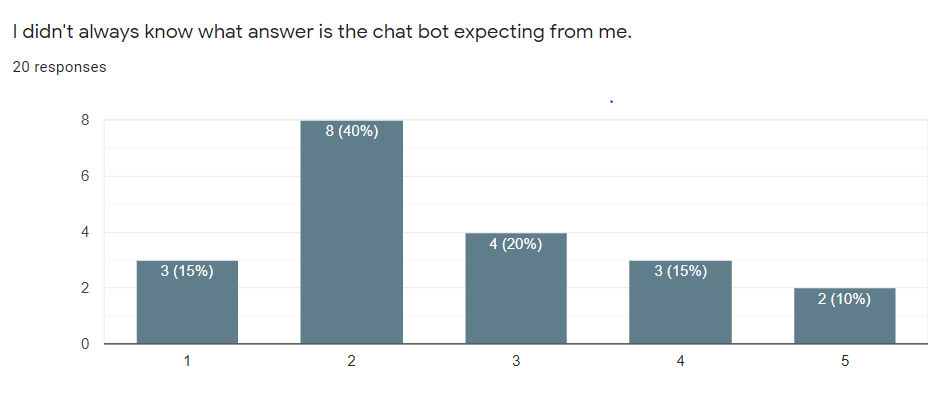
\includegraphics[width=0.9\textwidth]{img/Answer_Expect.PNG}
    \caption{Result for the users knowledge about the chatbot's expectation}
    \label{fig:ansExpec}
\end{figure}
\\~\\
Checking with the participants opinion about errors made by the chatbot and recovery from them, 9(45\%) stated that chatbot made errors. While 6(30\%) negated it and remaining 5(25\%) were unable to decide about it. But the positive point about the chatbot was, out of those users who faced the error or unable to decide about it during a chat, 10 of them were able to recover easily from the error. In addition to that, 12(60\%) of the participants rated the chatbot as cooperative. On contrary, just 4(20\%) marked it as uncooperative as portrayed in the Figure \ref{fig:cooperBot}.

\begin{figure}[!h]
    \centering
    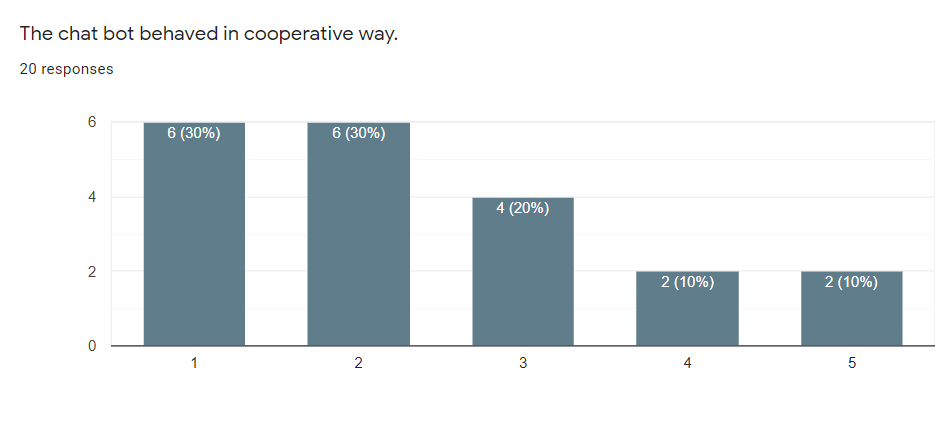
\includegraphics[width=0.9\textwidth]{img/Cooperative_Chatbot.PNG}
    \caption{Result about the the chatbot's cooperativity}
    \label{fig:cooperBot}
\end{figure}

\subsubsection*{Dialogue Assessment}
This part of the survey was added to judge the design of the dialogue according to the users perspective. Total six question were asked by the participants for completion of the purpose.
\begin{enumerate}
    \item I easily lost track of where I am in an interaction with the chat bot.
    \item The dialogue was bumpy.
    \item I was able to direct the conversation as desired.
    \item I felt in control of the interaction with the chat bot.
    \item The dialogue quickly led to the desired goal.
    \item The dialogue parts were evenly distributed between me an the chat bot.
\end{enumerate}
As plotted in the Figure \ref{fig:lostTrack} that 7(35\%) strongly disagreed while 6(30\%) simply disagreed with the statement that they lost the track during the communication with the chatbot. On the other hand, 6(30\%) were unable to make any decision and only 1(5\%) just agreed with it. So it can be concluded from the result analysis that maintaining a state for each module with respect to each user has been appeared really useful and effective.

\begin{figure}[!h]
    \centering
    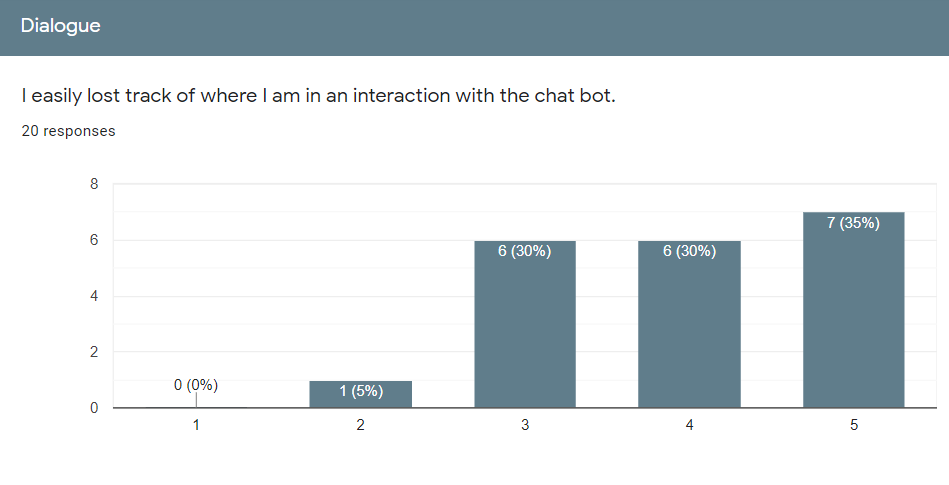
\includegraphics[width=0.9\textwidth]{img/Lost_Track.PNG}
    \caption{Result for users lost track during interaction with the chatbot}
    \label{fig:lostTrack}
\end{figure}
\\~\\
After analysing the results from the Figure \ref{fig:bumpDialo}, it is not wrong to say that the dialogue was smooth and communication between the users and the chatbot was comfortable and consistent. As, 10(50\%) of the participants showed disagreement with the statement that the dialogue was bumpy. Contrarily, only half of it that is 5(25\%) just find it unstable. Which means by using the modular architecture a stable and smooth dialogue can be designed.

\begin{figure}[!h]
    \centering
    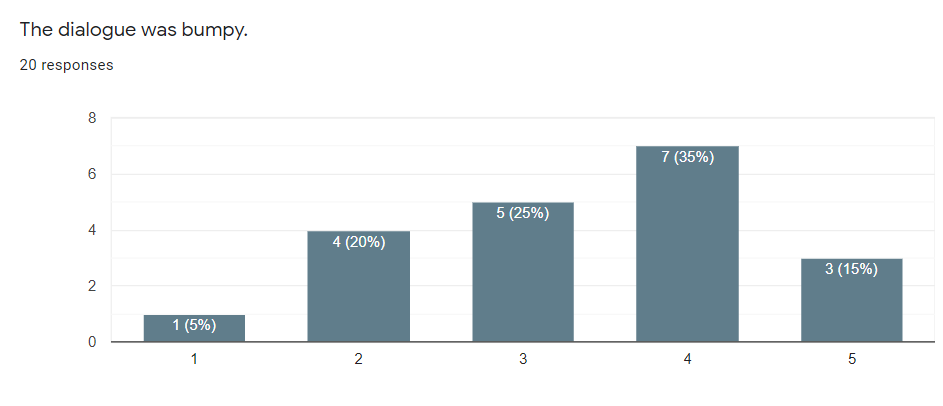
\includegraphics[width=0.9\textwidth]{img/Bumpy_Dialog.PNG}
    \caption{Result reflecting users opinion about bumpy dialogue}
    \label{fig:bumpDialo}
\end{figure}
\\~\\
Nextly, as presented in the Figure \ref{fig:desiredConv} that 8(40\%) of the participants were able to direct the conversation according to their desires. On the other hand, 6(30\%) out of the remaining 12 were unable to drive it according to their wish. And the left out 6(30\%) answered as undecided. And yet again the ratio of the respondents who were able to direct the conversation as desired appeared to be greater than the ones who were not be able to do it. As it was just simply a demo chatbot designed under various limitations of time and resources but still able to capture positivity out of the users. So, if the framework will undergo a proper training and design then it could be a revolutionary transformation for the chatbots.

\begin{figure}[!h]
    \centering
    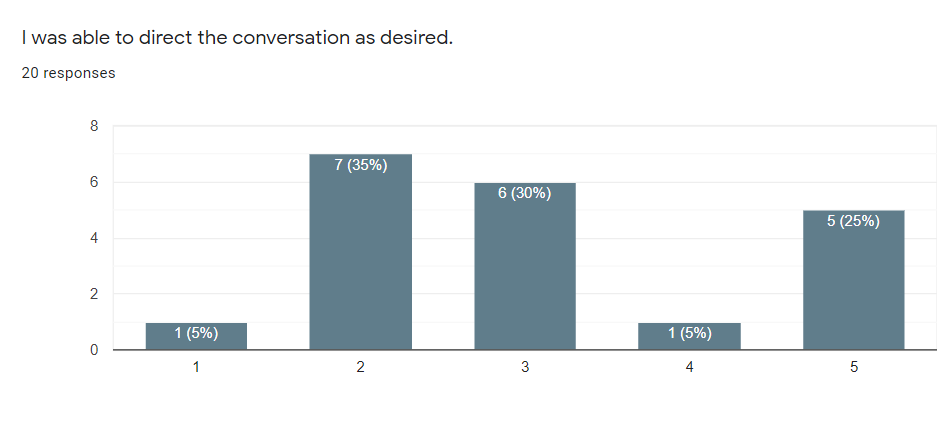
\includegraphics[width=0.9\textwidth]{img/Desired_Conv.PNG}
    \caption{Result reflecting users opinion about desired conversation}
    \label{fig:desiredConv}
\end{figure}
\\~\\
As shown in the Figure \ref{fig:chatbotControl}, that the number of participants who agreed and disagreed with the statement that they felt in control of the conversation with the chatbot is same and that is 6(30\%) for both categories. And remaining 8(40\%) were not able to decide about it. Now it is something alarming, as in this case the possible reason could be the topic of the demo chatbot. As I designed the detective chatbot and it was designed in a way to be a bit strict and commanding. 

\begin{figure}[!h]
    \centering
    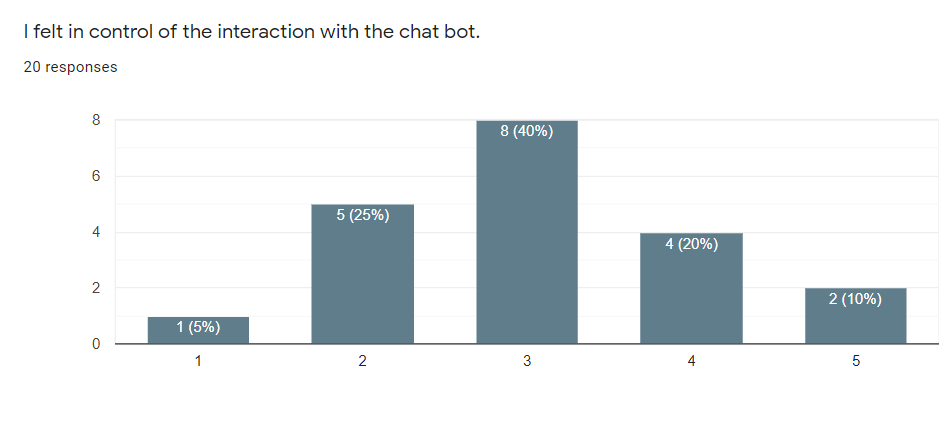
\includegraphics[width=0.9\textwidth]{img/Chatbot_Control.PNG}
    \caption{Result reflecting users opinion whether they felt that the chat was controlled by the chatbot}
    \label{fig:chatbotControl}
\end{figure}
\\~\\
According to the Figure \ref{fig:quickGoal}, 9(45\%) answered that the dialogue quickly led to the desired goal which refers to the fact that the detective game was designed in such manner that the user should be able to reach the final goal as quickly as possible. But also 7(35\%) disagreed with it and the cause behind it could be the wrong intent detection as user typed in something else but NLU recognized it differently due to which chatbot responded with some unrelated statement.

\begin{figure}[!h]
    \centering
    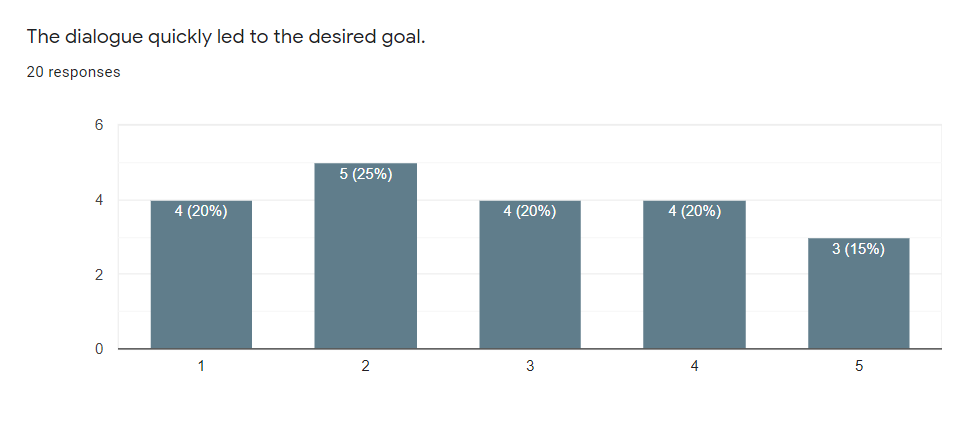
\includegraphics[width=0.9\textwidth]{img/Quick_Goal.PNG}
    \caption{Result reflecting users opinion about the dialogue quickly led to the goal}
    \label{fig:quickGoal}
\end{figure}
\\~\\
Referring to the Figure \ref{fig:evenDist}, 9(45\%) of the people who took part in to the study agreed with a statement that dialogue parts were equally distributed between them and the chatbot whereas, other 9(45\%) were leave it undecided and only 2(10\%) disagreed with it.

\begin{figure}[!h]
    \centering
    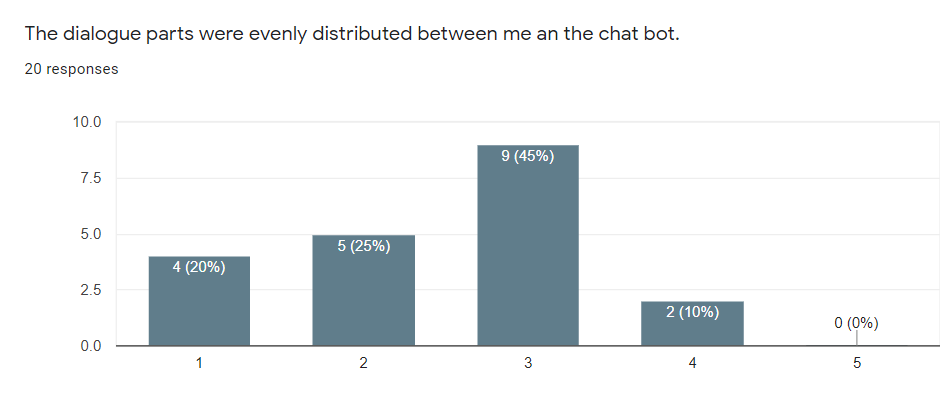
\includegraphics[width=0.9\textwidth]{img/Even_Parts.PNG}
    \caption{Result reflecting users opinion about the equal distribution of the dialogue parts}
    \label{fig:evenDist}
\end{figure}

\subsubsection*{Personal Experience and Impression}
This segment has been put to the questionnaire in order to collect users experience and personal impression about the chatbot. It also has been completed using series of questions. 
\begin{enumerate}
    \item The interaction with the chat bot was pleasant.
    \item I felt relaxed.
    \item High level of concentration is required while using the chat bot.
    \item The interaction was fun.
    \item Overall, I am satisfied with the chat bot.
    \item I felt that the chat bot was smart enough to handle the message which was not lying in its scope.
    \item I felt that the chat bot guided me well to return to the actual topic when I tried to misguide it.
    \item It was easy for me to continue the chat without any reluctance.
    \item It was easy for me to understand the response of the chat bot.
    \item It took me too long to make the chat bot understand my message by using different terms in sentences.
\end{enumerate}
As presented in the Figure \ref{}, majority of the participants i.e. 12(60\%) felt that the interaction with the chatbot was pleasant. It could be due to the reason that the user doesn't have to restart the chat whenever he/she wants to move to some different topic. The user was able to jump between different topics at any moment and can handle multiple topics at the same time without loosing the state for the last topic. 
\\~\\
According to the Figure \ref{}, 11(55\%) respondents responded that they felt relaxed while having a conversation with the chatbot. It was something important to make sure that chatbot is not making someone feel tensed or bad about anything. Furthermore, 10(50\%) of the users also showed disagreement to the statement that high level of concentration was required while using the chatbot. So, from this result it can be concluded that the chatbot and the dialogue design was simple and also user friendly. Additionally, 15(75\%) of the users found the interaction as fun. It was also the main purpose of the Frankenbot to entertain the users instead of making them feel nothing or bored. So, this purpose also gets accomplished. 
\\~\\
After analysing the result from the Figure \ref{} about the user satisfaction for the chatbot, it can be deduced that the majority of the users 10(50\%) felt satisfied with it. While, 5(25\%) out of the other 10 left it undecided and the remaining 5(25\%) were not satisfied with it.
\\~\\
Nextly, as figured out from the Figure \ref{}, majority 8(40\%) of the participants disagreed that the chatbot was able to handle the messages well which were out of its scope. Whereas, 7(35\%) of the respondents agreed with it. It happened surely due to the wrong recognition of the intent for the user utterance by the NLU. Otherwise, framework has been designed in such a manner that it should handle such scenario in well organized manner as already explained in the last chapter of this document. In addition to it, 14(70\%) of the respondents showed agreement to the statement that chatbot guided them well to return to the actual topic when they tried to misguide it. It makes the stance clear about the chatbot abilities that it has the skill to well manage the messages which do not lie under its scope provided enrich training data for NLU.
\\~\\
Moving to the next statement, 10(50\%) of the users agreed that they were able to continue the chat without any stoppage. It means the chatbot was working well for them as they wanted. The chatbot nor the user were reluctant to each other. It can also be concluded from this result that the dialogue was well structured and designed in order to perform smooth conversation without any objection or hesitation. Another important factor that can't be neglected is that the user should be able to understand the chatbot's response. So, 13(65\%) of the participants were able to do so. Which also marked this property as accomplished for the chatbot.
\\~\\
Lastly, 12(60\%) out of the total 20 participants negated the statement that it took them too long to make the chat bot understand their message by using different terms in sentences. It reflects that the information provided to the users was pretty much clear and also the guidance by the chatbot was enough for the user to enter correct answer.

\subsubsection*{Usability}
This part of the survey has been added to gather the users opinion about the chatbot's usefulness and whether it is easy to use or not. So, it has been judged on the basis of what users have answered to the following questions:
\begin{enumerate}
    \item The system is difficult to use.
    \item It is easy to learn to use the chat bot.
    \item The chat bot is too inflexible.
    \item I would like to use the chat bot again in the future.
    \item The chat bot operation was worthwhile.
\end{enumerate}
According to the result deduced from the Figure \ref{}, 15(75\%) of the users contradicted with the statement that the chatbot was difficult to use. Which means the majority of the participants found it easy to use. Additionally, again the same amount of the respondents i.e. 15(75\%) discovered that it was easier to understand the chatbot. It could be due to several reasons like the information provided was enough, the chatbot's ability to guide the user, structured dialogue and good understanding of the chatbot's response by the user.
\\~\\
Furthermore, 8(40\%) of the respondents disagreed with the statement that chatbot was too inflexible. Whereas, 7(35\%) showed agreement on this statement. This mixed opinion of user could be just because of the reason that the chatbot was designed in a way that it should guide the user to return to the actual topic instead of continuing the chat on any user's desired topic. As the chatbot has been trained using limited data, time and resources. Once, it will undergo good training then one can easily make it work for all user utterances regardless of the specific topic.
\\~\\
At the end, the users were asked whether they want to use the chatbot again in future. And 11(55\%) replied positively. Contrarily, only 4(20\%) responded negatively. Moreover, they were also asked to rate the chatbot's functioning whether it's worth the time and effort spent. And majority i.e. 11(55\%) of the participants agreed with it. On the other hand, only 4(20\%) of respondents disagreed with it.

\subsection{Evaluation via AttrakDiff}
The tool's single evaluation method has been used in order to judge the chatbot on the basis  of the following qualities:
\begin{itemize}
    \item Hedonic quality (joy of use, emphasized stimulation, identification and evocation generated by the system).
    \item Pragmatic quality (usefulness, efficiency, easy to use).
\end{itemize} 


